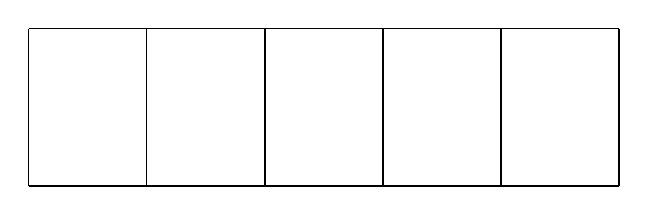
\begin{tikzpicture}[x=1cm,y=1cm,font=\normalsize,
 geometry edge/.style={solid,line width=.6pt},
 geometry mark/.style={solid,line width=.6pt},
 geometry label/.style={font=\normalsize,inner sep=2pt}]
\coordinate (T0) at (0.0000,2.0000);
\coordinate (B0) at (0.0000,0.0000);
\coordinate (T1) at (1.5000,2.0000);
\coordinate (B1) at (1.5000,0.0000);
\coordinate (T2) at (3.0000,2.0000);
\coordinate (B2) at (3.0000,0.0000);
\coordinate (T3) at (4.5000,2.0000);
\coordinate (B3) at (4.5000,0.0000);
\coordinate (T4) at (6.0000,2.0000);
\coordinate (B4) at (6.0000,0.0000);
\coordinate (T5) at (7.5000,2.0000);
\coordinate (B5) at (7.5000,0.0000);
\draw[geometry edge] (T0)--(T1);
\draw[geometry edge] (B0)--(B1);
\draw[geometry edge] (T1)--(T2);
\draw[geometry edge] (B1)--(B2);
\draw[geometry edge] (T2)--(T3);
\draw[geometry edge] (B2)--(B3);
\draw[geometry edge] (T3)--(T4);
\draw[geometry edge] (B3)--(B4);
\draw[geometry edge] (T4)--(T5);
\draw[geometry edge] (B4)--(B5);
\draw[geometry edge] (T0)--(B0);
\draw[geometry edge] (T1)--(B1);
\draw[geometry edge] (T2)--(B2);
\draw[geometry edge] (T3)--(B3);
\draw[geometry edge] (T4)--(B4);
\draw[geometry edge] (T5)--(B5);
\end{tikzpicture}
